\chapter{Customizable Contraction Hierarchies}\label{sec:Preliminary_CCH}

In this section we will present the basic idea of \cite[Customization Contraction Hierarchies]{CCH} and also work out the main difference between CCH and \cite[Contraction Hierarchies]{Geisberger_2012}.
It is far form being complete, but there will be some easy examples to show the concept. 

\section{Contracting}

\begin{algorithm}
    \caption{Insert Shortcuts Algorithm}
    \label{alg:contraction}
    \begin{algorithmic}[1]
    \Function{contractGraph}{V}
    \For{$v \in V$} 
        \State queue.offer(getContraction(v))
    \EndFor
    \While{queue is not empty}
    \State $\text{contraction} \gets \text{getContraction(queue.poll())}$
    \State $\text{v} \gets \text{contraction.v}$
    \State $\text{v.rank} \gets \text{rank}$
    \State updateNodeInNeo4J(vertex, rank++)
    \For{$shortcut \in contraction.shortcuts$}
        \State $\text{createOrUpdateEdge}(vertexToContract, shortcut)$
    \EndFor
    \For{$\text{neighbor} \in N_\downarrow(v) \cap N_\uparrow(v)$}
        \State $queue.update(getContraction(neighbor))$
    \EndFor
    \State \Return $v$
    \EndWhile
    \EndFunction

    \Function{getContraction}{v}
    \State$\text{shortcuts} \gets \text{[]}; \text{outerCount, innerCountTimesOuter} \gets 0$
    \For{$\text{inArc} \in \text{v.inArcs}$}
        \If{$\text{inArc.start.rank} = \text{Vertex.UNSET}$}
            \State $\text{outerCount++}; \text{inNode} \gets \text{inArc.start}$
            \For{$\text{outArc} \in \text{v.outArcs}$}
                \If{$\text{outArc.end}.rank = \text{Vertex.UNSET}$}
                    \State $\text{innerCountTimesOuter++; } \text{outNode} \gets \text{outArc.end}$
                    \If{$\text{inNode} \neq \text{outNode}$} $\text{shortcuts.add(Shortcut(inArc, outArc))} $ 
                    \EndIf
                \EndIf
            \EndFor
        \EndIf
    \EndFor
    \State $\text{ED} \gets |shortcuts| - outerCount -  (outerCount \text{ = 0 ? 0 : } \frac{innerCountTimesOuter}{outerCount})$
    \State \Return Contraction(v, ED, shortcuts)
    \EndFunction
    \end{algorithmic}
\end{algorithm}

\begin{figure}
    \centering
    \begin{tikzpicture}[node distance={15mm}, main/.style = {draw, circle}]

    \node[main] (x11) at (0, 0) {$3$};
    \node[main] (x21) at (1, 0) {$1$};
    \node[main] (x31) at (2, 0) {$5$};
    \node[main] (x41) at (3, 0) {$2$};
    \node[main] (x51) at (4, 0) {$4$};
    
    \draw (x11) -- (x21);
    \draw (x21) -- (x31);
    \draw (x31) -- (x41);
    \draw (x41) -- (x51);
    \draw[dashed, out=60, in=120] (x11) to (x31);
    \draw[dashed, out=60, in=120] (x31) to (x51);

    %------------------------------------------------

    \draw[dashed]  (6,0) -- (6,1.5);


    \node[main] (x3) at (8, 0) {$3$};
    \node[main] (x4) at (10, 0) {$4$};
    \node[main] (x5) at (9, 1) {$5$};

    \draw[ -Stealth] (x3) -- (x5);
    \draw[ -Stealth] (x5) -- (x4);
    

\end{tikzpicture}
    \caption{The numbers inside the vertices represent their contraction order}
    \label{fig:contrating_and_searching}
\end{figure}

Algorithm \ref{alg:contraction} provides our contraction algorithm. We do what is called a \textit{metric dependent} contraction in \cite[Customization Contraction Hierarchies]{CCH}. 
This is a greedy algorithm which always takes the next best vertex to contract. Some use the simple edge difference as \cite[Contraction Hierarchies]{Geisberger_2012}, but we will use
a more advanced metric as desired in 

\subsection{Example}

In Figure \ref{fig:contrating_and_searching} you can see a contracted graph $G'(V,E')$ on the left. The solid lines represent the original edges $E$ of a graph $G$. The dashed lines between vertices are shortcuts $S$ that 
have been added while creating the CCH index graph G'(V, E'). The numbers inside the vertices reflect the contraction order.
\\
Contracting a vertex means deleting it. While contracting a vertex we want to preserve its via connection. If a vertex that is contracted resides on a simple path between two vertices of higher rank,
and there is no edge $e \epsilon E'$ between these vertices a shortcut has to be inserted between the two. 
Let's reconstruct the contraction of Figure \ref{fig:contrating_and_searching}. At first vertex $v(1)$ is removed. As $v(1)$ resides on a simple path to between $v(3)$ and $v(5)$ and there is no edge $e(v(3), v(5)) \notin E'$,
there must be a shortcut added to keep the via path.
The same applies after contracting $v(2)$ for the vertices $v(4)$ and $v(5)$. For all the other vertices we do not need to insert shortcuts.

\section{Searching}

\begin{algorithm}
    \caption{Find Search Path}
    \label{alg:cchSearch}
    \begin{algorithmic}[1]
    \Function{find}{$\text{start}, \text{goal}$}
        \State $\text{pickForward} \gets \text{true};$ $\text{forwardQuery} \gets \text{Query}(\text{start});$$\text{backwardQuery} \gets \text{Query}(\text{goal});$
        \While{not \Call{isComplete}{$\text{forwardQuery, backwardQuery, candidates.peek()}$}}
            \State $\text{query} \gets \text{pickForward} ? \text{forwardQuery} : \text{backwardQuery}$
            \State $\text{other} \gets \text{pickForward} ? \text{backwardQuery} : \text{forwardQuery}$
            \State $\text{pickForward} \gets \neg \text{pickForward}$
            \If{\Call{isNotComplete}{$\text{query}$}}
                 $\text{query.expandNext()}$
            \Else
                 \textbf{ continue}
            \EndIf            
            \State $\text{latest} \gets \text{query.latestExpand()}$
            \If{$\text{other.resultMap().containsKey}(\text{latest.rank})$}
                \State $\text{forwardPath} \gets \text{forwardQuery.getPath}(\text{latest.rank})$
                \State $\text{backwardPath} \gets \text{backwardQuery.getPath}(\text{latest.rank})$
                \State $\text{candidates.offer}(\text{forwardPath} + \text{backwardPath})$
            \EndIf
        \EndWhile
        \State \Return $\text{candidates.poll()}$
    \EndFunction

    \Procedure{expandNext()}{}
    \State $\text{state} \gets \text{queue.poll()}$
    \State $\text{latestExpand} \gets \text{state}$
    
    \If{$\text{goals.contains}(\text{state.getEndVertex().rank}) $}
        \State $\text{shortestPaths.put}(\text{state.getEndVertex().rank}, \text{state.getPath()})$
    \EndIf
    \State $\text{state.settle()}$
    \For{ $\text{arc} \ \text{in} \ \text{state.getEndVertex().arcs}$}
        \State $\text{neighbor} \gets \text{arc.otherVertex}(\text{state.getEndVertex()})$
        \If{\Call{mustUpdateNeighborState}{$\text{state, neighbor, arc.weight}$}}
        \State $\text{newState} \gets \text{state.getPath()} + \text{arc}$
        \State $\text{queue.update}(\text{State}(\text{neighbor, newState}))$
        \State $\text{seen.put}(neighbor.rank, newState)$
            
        \EndIf
    \EndFor
    \EndProcedure
    \end{algorithmic}
\end{algorithm}

some text

\subsection{Example}

As we preserved all via paths during the contraction the shortest path can be retrieved by a bidirectional Dijkstra that is restricted such that it only expands vertices of higher rank. 
Therefore if one wants to retrieve the shortest path between $v(3)$ and $v(4)$ there will be a forward search from $v(3)$ and a backward search from $v(4)$. As we restrict theses searches to expand only vertices
of higher rank, the only vertices to expand are the start and target vertex. Both will find only one vertex $v(5)$, the highest vertex and the meeting point, too. Finding at least one meeting point in the forward an backward search means there exist a path between them.
After merging these paths at the middle vertex $v(5)$ one will obtain the shortest path.
\\
For an arbitrary contracted graph is it possible that there are more than one meeting point. As merging two shortest paths will not necessary lead to an other shortest path, one has to merge
all possible meeting points and take the path among the merged ones which has the smallest distance. 
\\ 
The stopping condition for such a CH-Search is either, both forward and backward search, have reached the top vertex so there is no further vertex to expand, which happens in the example of figure \ref{fig:contrating_and_searching} or, backward and forward search exceed 
the length that has already been found among the merged paths.


\section{Difference between CH and CCH}

Looking at the left graph in Figure \ref*{fig:DifferenceCHAndCCH} it has been contracted in the CH way, whereas the right is the CCH way. We explicitly state this here because 
we have found paper \cite{Ouyang_2020} that mix up these well known names, claiming they to Contraction Hierarchies CH while actually doing Customizable Contraction Hierarchies CCH. 
The main difference is, CH will only insert an shortcut between two vertices if the vertex that is contracted resides on the shortest path between two of its neighbors. 
When vertex $v(1)$ is contracted there is no shortcut inserted as vertex $v(1)$ is not on the shortest path between which is via vertex $v(4)$.
\\
Whereas in the CCH case the edge weights do not play a role a contraction time. If a vertex is contracted and there is no direct connection between two of its neighbors, one has to insert a shortcut. This gives
the advantage that later on we can easily update edge weights without inserting new shortcut, as all possibly needed shortcuts already exist.
\\ 
Let's complete this example by updating the edge $e(v(2), v(4))$ that currently has the weight of $w(e)=1$ to $w(e) = 5$. Now the vertex $v(1)$ is on the shortest path between vertex $v(2)$ and $v(3)$. 
To update the CH graph we have to insert an edge between vertex $v(2)$ and $v(3)$ whereas the topological structure of the CCH remains the same, one only need to update the weight and the middle vertex of the already give shortcut edge.

\begin{figure}
    \centering
    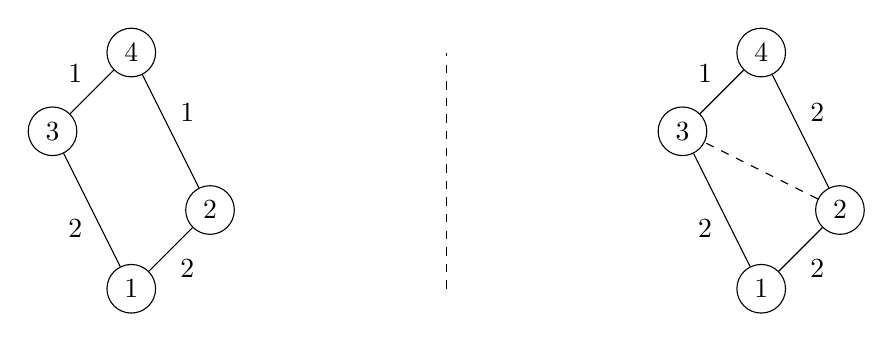
\begin{tikzpicture}[node distance={15mm}, main/.style = {draw, circle}]

    \node[main] (x3) at (0, 2) {$3$};
    \node[main] (x4) at (1, 3) {$4$};
    \node[main] (x2) at (2, 1) {$2$};
    \node[main] (x1) at (1, 0) {$1$};
    
    \draw (x1) -- node[below right] {$2$}(x2);
    \draw (x1) -- node[below left] {$2$} (x3);
    \draw (x2) -- node[above right] {$1$} (x4);
    \draw (x3) -- node[above left] {$1$} (x4);

    \draw[dashed]  (5,0) -- (5,3);

    \node[main] (x31) at (8, 2) {$3$};
    \node[main] (x41) at (9, 3) {$4$};
    \node[main] (x21) at (10, 1) {$2$};
    \node[main] (x11) at (9, 0) {$1$};
    
    \draw (x11) -- node[below right] {$2$}(x21);
    \draw (x11) -- node[below left] {$2$} (x31);
    \draw (x21) -- node[above right] {$2$} (x41);
    \draw (x31) -- node[above left] {$1$} (x41);
    \draw[dashed] (x21) -- node[above, sloped] {}  (x31);

    
\end{tikzpicture}
    \caption{The left represents a CH and the right a CCH contracted graph}
    \label{fig:DifferenceCHAndCCH}
\end{figure}

\section{Metric Dependent Vertex Order}\label{sec:metric_dependent_vertex_order}
There are two ways to get a suitable vertex order. A so called \textit{metric independent} and a so called \textit{metric dependent} one. The metric independent recursively uses balanced separator to determine a vertex ordering\cite{CCH}. Although this is the superior method, it is not used in this paper writing an algorithm that calculates balanced separators isn't trivial, and we are not aiming for optimizing the contraction process. 
The metric dependent order mainly uses the edge difference $ED$ to determine which vertex is to be contracted next. The $ED$ is determined as the $|edges To Insert| - |edges To Remove|$. The fewer edges are inserted during contraction the fewer edges will be contained by the final graph, therefore fewer edges to expand in a search. However using only the edge differences doesn't lead to desired result. This is because during contraction there will be areas that get less dense than others. 
There are two problems that can arise. One is that important vertices are not contracted last. The other is the search space of the query gets linear although it could be logarithmic.

\subsection{Important Vertices not contracted last}\label{sec:not_contracted_last}

\begin{figure}
    \centering
    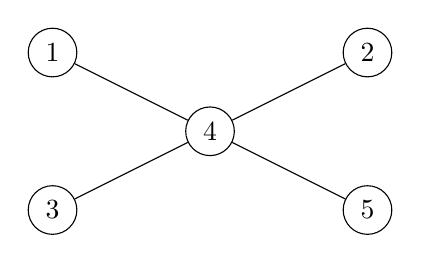
\begin{tikzpicture}[node distance={15mm}, main/.style = {draw, circle}]
    \node[main] (x1) at (1, 2) {$1$}; 
    \node[main] (x3) at (1, 0) {$3$};
    
    \node[main] (x4) at (3, 1) {$4$}; 
    
    \node[main] (x2) at (5, 2) {$2$}; 
    \node[main] (x5) at (5, 0) {$5$}; 
    
    \draw (x1) -- (x4);
    \draw (x2) -- (x4);
    \draw (x3) -- (x4);
    \draw (x5) -- (x4);
    
\end{tikzpicture} 
    
    \caption{The numbers inside the vertices represent their contraction order}
    \label{fig:not_contracted_last}
\end{figure}

Looking at figure \ref{fig:not_contracted_last}, this is a possible contraction order, if only the $ED$ is used to contract vertices. At the beginning the vertices with rank 1, 2, 3, 5 have the same edge difference, which is $ED = -1$. Vertex after vertex is removed  and  no shortcut is inserted. This happens until there are only $v(4)$ and $v(5)$ left. Now $v(4)$ has an $ED=-1$, too, same as vertex 5. Therefore the algorithm contracts $v(4)$ before $v(5)$. However this is not the desired result. There are six \\$e(v(1),v(2)), e(v(1),v(3)), e(v(1),v(5)), e(v(2),v(3)), e(v(2),v(5)), e(v(3),v(5))$  shortest paths that involve  $v(4)$, all the other vertices do not encode any shortest path, so $v(4)$ should be contracted last. The search graph on the right of Figure \ref{fig:not_contracted_last} shows why. Imagine we we do a shortest path query between $v(1)$ and $v(3)$. After expanding both, the forward and the backward search to $v(4)$, there is yet another vertex we'll have to expand $v(5)$. Although 
as you can see in the original graph on the right, its not possible that $v(5)$ is on the shortest path. Therefore a better contraction order would be a in Figure \ref{fig:contrating_and_searching}.  This can be overcome by the method that is explained in section \ref{sec:vertex_importance}.

\subsection{Linear Query Search Space}\label{sec:linear_query}

\begin{figure}
\centering
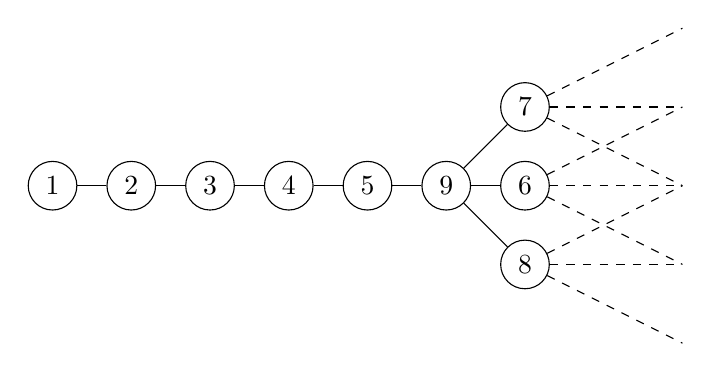
\begin{tikzpicture}[node distance={15mm}, main/.style = {draw, circle}]

    \node[main] (x1) at (0, 0) {$1$};
    \node[main] (x2) at (1, 0) {$2$};
    \node[main] (x3) at (2, 0) {$3$};
    \node[main] (x4) at (3, 0) {$4$};
    \node[main] (x5) at (4, 0) {$5$};
    \node[main] (x9) at (5, 0) {$9$};
    
    \node[main] (x7) at (6, 1) {$7$};
    \node[main] (x8) at (6, -1) {$8$};
    \node[main] (x6) at (6, 0) {$6$};
    
    
    \draw (x1) -- (x2);
    \draw (x2) -- (x3);
    \draw (x3) -- (x4);
    \draw (x4) -- (x5);
    \draw (x5) -- (x9);
    
    \draw (x6) -- (x9);
    \draw (x9) -- (x7);
    \draw (x9) -- (x8);
    
    \draw [dashed] (x7) -- (8, 2);
    \draw [dashed] (x7) -- (8, 1);
    \draw [dashed] (x7) -- (8, 0);
    
    \draw [dashed] (x8) -- (8, 0);
    \draw [dashed] (x8) -- (8, -2);
    \draw [dashed] (x8) -- (8, -1);
    
    \draw [dashed] (x6) -- (8, 1);
    \draw [dashed] (x6) -- (8, 0);
    \draw [dashed] (x6) -- (8, -1);
    
\end{tikzpicture} 
    
\caption{Linear Contraction}
\label{fig:linear_contraction}
\end{figure}

Regarding figure \ref{fig:linear_contraction} there are three possible index graphs $G'$ of one and the same base graph $G$. The numbers inside the vertices represent the contraction order.
\\
The first one could be contracted using the edge difference $ED$, as always one of the outer vertices with $ED=-1$ was contracted. On the one hand it reaches the optimum in case for \textit{least shortcuts inserted}. On the other though it has the worst search space among the three vertex orderings. 
To get from vertex $v(1)$ to $v(5)$ we have to expand four vertices. 
\\
The second $G'$ one contracts the middle vertices, which encodes the most shortest paths, first and therefore inserts three shortcuts. Although this example has a lot of shortcuts, there are still a lot of vertices to expand in some cases. In case every vertex of $G$ has a weight of $1$, and one wants to go from $v(1)$ to $v(5)$ the forward search will have to expand four vertices as in the upper first example.
\\
The third example contracts the middle vertex last. At first it contracts the vertices right next to the middle vertex. Therefore we have to insert shortcuts between $e(v(3)v(5))$ and $e(v(4), v(5))$,
so no matter what source, target pair we are trying to find in this example, the forward and the backward search will have to expand at most one single vertex. This example additionally shows that
recursively finding a balanced separator, as proposed in \cite[Customization Contraction Hierarchies]{CCH}, is very a promising method to obtain a good contraction order. 

\section{Vertex importance}\label{sec:vertex_importance}

As shown in section \ref{sec:not_contracted_last} and \ref{sec:linear_query} there are vertices that are more important that other vertices. Contracting these vertices late is key to get a efficient search later on. 

\subsection{Suitability of CCH}

As it is important to contract important vertices last, the advantage one gets making a CCH search over a simple dijkstra run depends whether the base graph $G(V, E)$ has vertices that are more important than others. 
A vertex $v \epsilon E$ is important if there a many shortest paths that contain this very vertex. Therefore if it is possible to calculate a small balanced separator on $G$, CCH will be able to show its 
whole advantage. To dive deeper into this topic, have a look at \cite[Lower Bounds and Approximation Algorithms for Search Space Sizes in Contraction Hierarchies]{BlumStorandt}.

\subsection{Metric dependent Importance}

As shown above, taking only the edge difference $ED$ into account doesn't necessarily lead to a proper order, we decided to take the vertex importance calculation that is propose by \cite[Customization Contraction Hierarchies]{CCH}. To every 
vertex we add the level property $l(v)$. The level of the vertex with is initially set to $0$. If a neighbor $w = N(v)$ is contracted level is set to $l(v) = max\{l(v)+1, l(w)\}$. For every arc $a \epsilon A'$
we add a the hop length to the arc $h(a)$. The hop length is equals the number of arcs, this arc represent when fully unpacked. Additionally, we denote as $A(v)$ the set of inserted arcs after the contraction
of $v$ and $D(v)$ the set of removed arcs. We calculate the importance $i(v)$ as follows:

\begin{equation*}
    i(v) = l(v) + \frac{|A(v)|}{|D(v)|} + \frac{\sum_{a \epsilon A(v)} h(a)}{\sum_{a \epsilon D(v)} h(a)} 
\end{equation*}

Our tests show that this importance calculation result in slightly increase in the amount of shortcuts added, but the maximum Vertex degree is smaller. Which speeds up the contraction process towards the end. Additionally
the average search time decreases as the search space decreases too. 

% \section{Perfect Customization}
% 
% \begin{figure}
    % \centering
    % 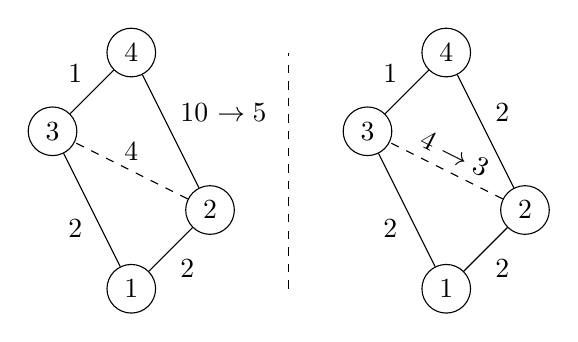
\begin{tikzpicture}[node distance={15mm}, main/.style = {draw, circle}]

    \node[main] (x3) at (0, 2) {$3$};
    \node[main] (x4) at (1, 3) {$4$};
    \node[main] (x2) at (2, 1) {$2$};
    \node[main] (x1) at (1, 0) {$1$};
    
    \draw (x1) -- node[below right] {$2$}(x2);
    \draw (x1) -- node[below left] {$2$} (x3);
    \draw (x2) -- node[above right] {\sout{$10$} $\rightarrow 5$} (x4);
    \draw (x3) -- node[above left] {$1$} (x4);
    \draw[dashed] (x2) -- node[above] {$4$} (x3);

    \draw[dashed]  (3,0) -- (3,3);

    \node[main] (x31) at (4, 2) {$3$};
    \node[main] (x41) at (5, 3) {$4$};
    \node[main] (x21) at (6, 1) {$2$};
    \node[main] (x11) at (5, 0) {$1$};
    
    \draw (x11) -- node[below right] {$2$}(x21);
    \draw (x11) -- node[below left] {$2$} (x31);
    \draw (x21) -- node[above right] {$2$} (x41);
    \draw (x31) -- node[above left] {$1$} (x41);
    \draw[dashed] (x21) -- node[above, sloped] {\sout{$4$} $\rightarrow 3$}  (x31);

    
\end{tikzpicture}
    % \caption{Perfect Customization}
    % \label{fig:perfectCustomization}
% \end{figure}

\section{Update CCH}

\begin{algorithm}
    \caption{Update}
    \begin{algorithmic}[1]
    
    \Procedure{update()}{$G$}
    \State $\text{Q} \gets$ $G'.updatedEdges(G)$; 
    \While{$Q \neq \emptyset $}
        \State $a \gets Q.poll()$; 
        \State $oldWeight \gets w(a)$
        \State $newWeight \gets determineNewWeight(a)$
        \If{$oldWeight != newWeight$}
            \State $w(a) \gets newWeight$
            \State $checkTriangles(Q, oldWeight, upperTriangles(a))$
            \State $checkTriangles(Q, oldWeight, intermediateTriangles(a))$
        \EndIf
    \EndWhile
    \EndProcedure

    \Procedure{checkTriangles}{$Q, oldWeight, triangles$}
    \ForAll{$triangle$ in $triangles$}
        \If{$triangles.c() == triangle.b() + oldWeight$}
            \State{Q.push(triangle.c())}
        \EndIf
    \EndFor
    \State \textbf{return} $\text{triangles}$
    \EndProcedure
        
    \end{algorithmic}
\end{algorithm}

The biggest advantage of CCH over CH is, that it is easy to update without the need of changing the topological structure of the index graph. This is the reason why CCH can be interesting for graph databases.
If an arcs $w(a(x, y))$ weight increases or decreases this can result in a weight change on arcs that connect vertices of higher rank than $x, y$. We determine all arcs of the input graph $G$ that have been changed 
and push them to a priority queue. The queue always pops the the arc $a(x,y)$ with the lowest rank of the start vertex $x$. If there are multiple it pops the one with the lowest rank of $y$ among the ones with the lowest rank of $x$. Then we determine 
the new weight of the arc using the lower triangles. If there is a lower triangle that can be used as a pass through such that the arc weight in $G'$ does not change we do nothing. If the weight of the arc has changed
we assign the new weight to the arc. Then we check all upper triangles, as drawn in figure \ref{fig:updateTriangles}, of $a(x,y)$ if there is an upper arc; denoted by $c$ in figure \ref{fig:updateTriangles}, that is influenced by this very change. If it is influenced by this
change we push it to the priority queue. We do the same with all intermediate triangles. 
\\


\begin{figure}
    \centering
    \begin{tikzpicture}[node distance={15mm}, main/.style = {draw, circle}]

    \node[rotate=90] at (-0.25,0) {rank};
    \draw [ -Stealth]  (0,-2) -- (0,2);

    \node[] at (3,3) {Intermediate Triangles};
    
    \node[main] (z2) at (1, 0) {$z$}; 
    \node[main] (x2) [below right of=z2] {$x$};
    \node[main] (y2) [right of=z2, above of=z2] {$y$}; 
    \draw[ -Stealth] (z2) -- node[above left, sloped] {$c$} (y2);
    \draw[ -Stealth] (z2) -- node[below left, sloped, pos=0.8] {$b$} (x2);
    \draw[ -Stealth] (x2) -- node[below left, sloped] {$a$} (y2);
    \node[] at (2,-2) {$c_\uparrow = a_\uparrow + b_\downarrow $};
    
    \node[main] (z21) at (4, 0) {$z$}; 
    \node[main] (x21) [below right of=z21] {$x$};
    \node[main] (y21) [right of=z21, above of=z21] {$y$}; 
    \draw[ -Stealth] (y21) -- node[above , sloped] {$c$} (z21) ;
    \draw[ -Stealth] (x21) -- node[below right, sloped, pos=0.8] {$b$} (z21);
    \draw[ -Stealth] (y21) -- node[below left, sloped] {$a$} (x21);
    \node[] at (5,-2) {$c_\downarrow = a_\downarrow + b_\uparrow $};

    \node[] at (11,3) {Upper Triangles};
    
    \node[main] (y3) at (9, 0) {$y$}; 
    \node[main] (x3) [below right of=y3] {$x$};
    \node[main] (z3) [right of=y3, above of=y3] {$z$}; 
    \draw[ -Stealth] (z3) -- node[above , sloped] {$c$} (y3);
    \draw[ -Stealth] (x3) -- node[below right, sloped, pos=0.8] {$a$} (y3);
    \draw[ -Stealth] (z3) -- node[below left, sloped] {$b$} (x3);
    \node[] at (10,-2) {$c_\downarrow = a_\uparrow + b_\downarrow$};

    \node[main] (y3) at (12, 0) {$y$}; 
    \node[main] (x3) [below right of=y3] {$x$};
    \node[main] (z3) [right of=y3, above of=y3] {$z$}; 
    \draw[ -Stealth] (y3) -- node[above left, sloped] {$c$} (z3);
    \draw[ -Stealth] (y3) -- node[below left, sloped, pos=0.8] {$a$} (x3);
    \draw[ -Stealth] (x3) -- node[below left, sloped] {$b$} (z3);
    \node[] at (13,-2) {$c_\uparrow = a_\downarrow + b_\uparrow$};

\end{tikzpicture}
    \caption{Update Triangles}
    \label{fig:updateTriangles}
\end{figure}